\documentclass[11pt,a4paper]{scrartcl}

\usepackage[utf8]{inputenc}
\usepackage[T1]{fontenc}
\usepackage[english]{babel}
\usepackage[babel,german=quotes]{csquotes}
\usepackage[pdftex]{graphicx}
\usepackage{amsmath,amssymb,amsthm}
\usepackage{latexsym}
\usepackage{hyperref}
\usepackage{import}
\usepackage{subcaption}
\usepackage{graphicx}
\usepackage{caption}

\newcommand{\Fig}[0]{Fig.}
\newcommand{\Eq}[0]{Eq.}

\hypersetup{
	pdftitle={CNN for plot function detection},
	pdfsubject={Applied Machine Learning Group Project},
	pdfauthor={Philipp Fürst},
	pdfkeywords={wissenschaftliches Schreiben}
}
\usepackage[anythingbreaks]{breakurl}
\usepackage{listings}
\lstset{numbers=left,
	numberstyle=\small,
	numbersep=5pt,
	breaklines=true,
	showstringspaces=false,
	frame=1 ,
	xleftmargin=15pt,
	xrightmargin=15pt,
	basicstyle=\ttfamily\scriptsize,
	stepnumber=1,
	keywordstyle=\color{ao}\textbf,         
  	commentstyle=\color{gray},       
  	stringstyle=\color{mauve}         
}
\lstloadlanguages{TeX}

\usepackage{color}
\definecolor{ao}{rgb}{0.0,0.0,1.0}
\definecolor{dkgreen}{rgb}{0,0.6,0}
\definecolor{gray}{rgb}{0.5,0.5,0.5}
\definecolor{lightgray}{rgb}{0.8,0.8,0.8}
\definecolor{mauve}{rgb}{0.58,0,0.82}

\usepackage[backend=biber]{biblatex} 
\ExecuteBibliographyOptions{
sorting=nyt, 
bibwarn=true, 
isbn=false, 
url=false 
}
\addbibresource{literatur.bib} 

\setlength{\topmargin}{-10mm}

\begin{document}
	\lstset{language=tex}
	
	\pagenumbering{roman}
	\pdfbookmark{Title page}{titlepage}
	\begin{titlepage}
		 \center
		 
\includegraphics[scale=0.2]{ImageFiles/unistuttgart_logo_de} 
		 \vspace*{2cm} 
		
		\begin{center} \large 
		     
			 \vspace*{2cm}
			 {\huge \textbf{CNN for plot function detection}}
			 \vspace*{2.5cm}
			
			 Applied Machine Learning Group Project
			 \vspace*{2.5cm}
			
			 Philipp Fürst (3383656)\\
			 Wasim Essbai (3649361)
			 \vspace*{1cm}
		\end{center}
	\end{titlepage}

	\tableofcontents
	\listoffigures
	\listoftables
	\pagebreak
	
	\pagenumbering{arabic}
  	\pagestyle{plain}
  
	\section{Introduction}
	The aim of this project is to design a machine learning model able to recognize a mathematical function from its graph. This is showed in \Fig~\ref{fig:GeneralIdea}.
	\begin{figure}[h!]
		\centering
		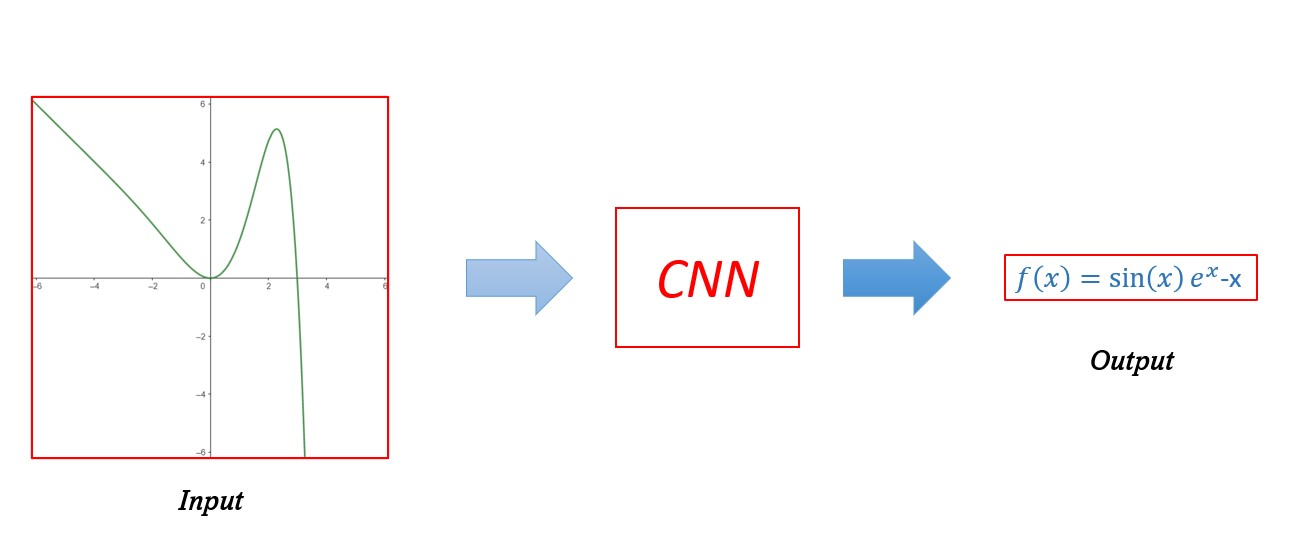
\includegraphics[width=0.7\linewidth]{./ImageFiles/general_idea}
		\caption{Final result to achieve}
		\label{fig:GeneralIdea}
	\end{figure}\\This problem can be approached as an image classification task.A common method for solving this type of problem is to use Convolutional Neural Networks (CNN).

	\section{Data Generation}
	Neural Networks models need a large amount of training data. The first challenge was to retrieve that data.\\
	For this project we developed an algorithm to generate and classify data, since no graph function datasets were available. This algorithm allowed to retrieve an arbitrary large amount of data. It is described in the following section.
	
	\import{./TextFiles/Data Generation/}{Algorithm.tex}
	\import{./TextFiles/Data Generation/}{Plots.tex}
	\import{./TextFiles/Data Generation/}{Labeling.tex}


	\section{CNN model}
	\import{./TextFiles/CNN/}{Architecture.tex}
	\import{./TextFiles/CNN/}{Implementation.tex}
	
	\section{Data Processing \& Training}
	\import{./TextFiles/Training/}{Data Processing.tex}
	\import{./TextFiles/Training/}{Training.tex}

	\section{Experimental Results}
	From the obtained model, the accuracy is 0.3\% for both training and validation data. The perfomances are very poor, but doing more analysis it can be seen that the performances increases a lot comparing sub-vectors. More precisely, the comparison is made for all components except the first $n_{shift}$ entries, that could be considered less relevant, since more deeper in the computational graph.\\
	This was done on test data, with output size 7, that were never used before, obtaining the values in table \ref{table:accshift}.
	It's possible to see that the network learned how to classify images except the first two entries.
		\begin{table}[h!]
		\centering
		\begin{tabular}{c|c c c}
			\hline
			$n_{shift}$ & 0 & 2 & 4\\
			\hline
			Accuracy & 0.4\% & 25.89\% & 86.41\%
		\end{tabular}
		\caption{Accuracy vs shift comparison}
		\label{table:accshift}
	\end{table}\\
	After a review of the work done, two main candidate reasons came out:
	\begin{enumerate}
		\item Image representation: The main problem is the presence of different ways to express the same mathematical function that are not managed yet, e.g. $f(x) = \log(e^x)$ and $f(x) = x$ are equivalent but with different encoding.
		\item Not suitable CNN architecture, that does not allow to achieve low training loss. Different architecture should be explored.
		\item Regression approach: The problem is basically a classification task, but, due to the hight number of possible classes, a regression approach was done in order to overcome that limit. This was a first approach, but with different approaches it might be possible to imporove significantly.
	\end{enumerate}
	\section{Conclusions}
	The general idea of this project has demonstrated to work, with still significant limits.\\
	Furthermore, for computational resources, the dataset size is kept low with respect to the number of possible classes. Ongoing work could focus on the limits presented in the previous section, but the model demonestrated some learning capabilities.
\end{document}